\chapter{Capturas de la Interfaz de Usuario} \label{ch:anexoA}

\section{Interfaz de Estadísticas}

Cada una de las estadísticas ha sido diseñada de manera independiente y autocontenida. Es por esto por lo que, aunque se sigan las directrices de diseño generales de la página, cada una tiene un caracter y presentación diferenciable. También cabe destacar que, en algunas de ellas, se ha preferido desarrollar la implementación funcional de manera más robusta, antes de invertir el tiempo en mejorar por completo la estética de la presentación.

\begin{figure}[H]
    \centering
    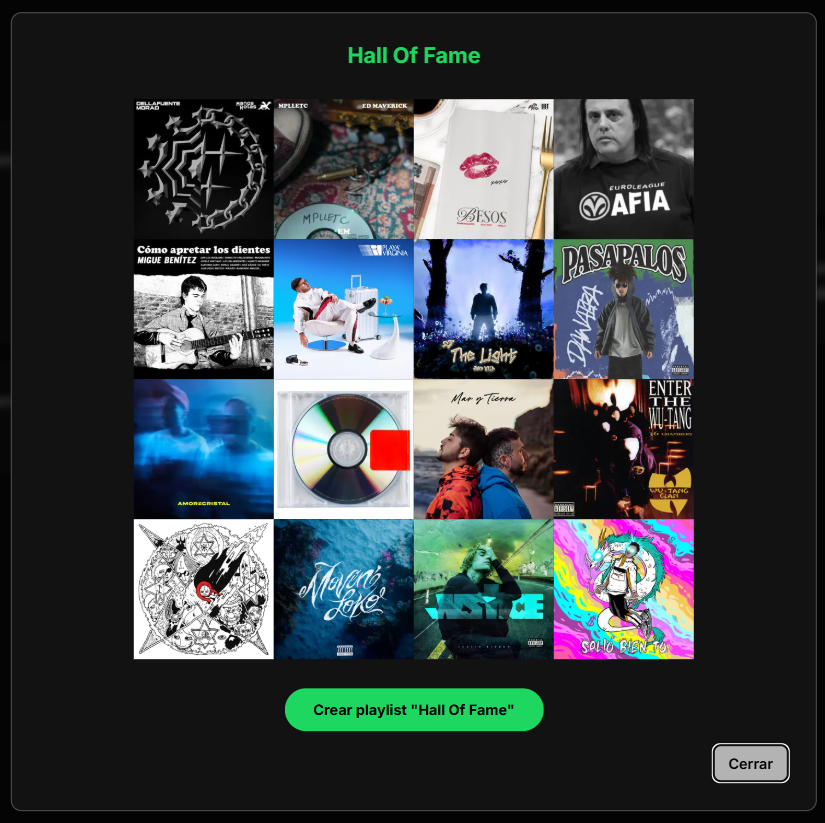
\includegraphics[width=0.45\textwidth]{figures/capturas_ui/hall_of_fame.png}
    \caption{Interfaz de la estadística \textit{Hall Of Fame}.}
    \label{fig:hall_of_fame}
\end{figure}

\begin{figure}[H]
    \centering
    \vspace{-10pt}
    \begin{minipage}{0.32\textwidth}
        \centering
        \includegraphics[width=\textwidth]{figures/capturas_ui/la_bitacora_año.png}
        \caption{Interfaz de la estadística \textit{La Bitácora} (año).}
        \label{fig:la_bitacora_año}
    \end{minipage}
    \begin{minipage}{0.32\textwidth}
        \centering
        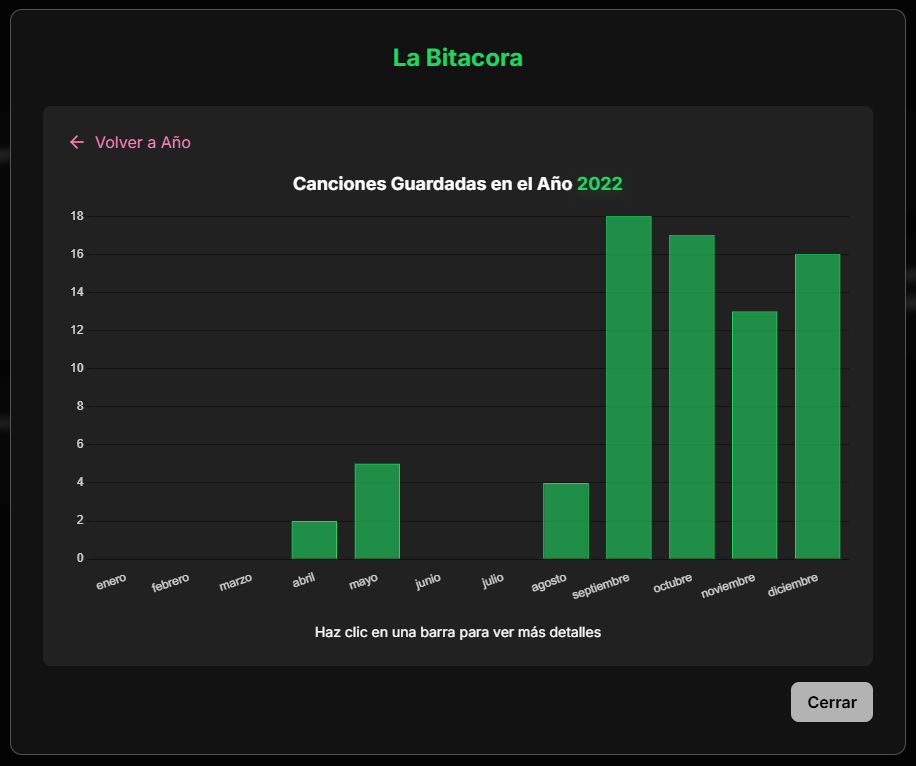
\includegraphics[width=\textwidth]{figures/capturas_ui/la_bitacora_mes.png}
        \caption{Interfaz de la estadística \textit{La Bitácora} (mes).}
        \label{fig:la_bitacora_mes}
    \end{minipage}
    \begin{minipage}{0.32\textwidth}
        \centering
        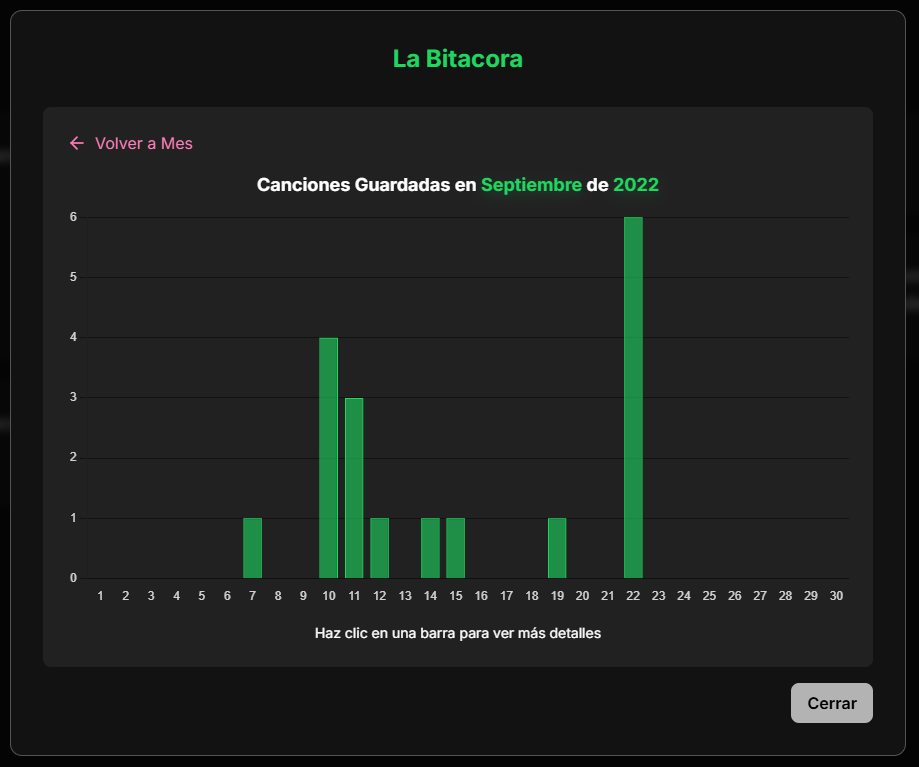
\includegraphics[width=\textwidth]{figures/capturas_ui/la_bitacora_dia.png}
        \caption{Interfaz de la estadística \textit{La Bitácora} (día).}
        \label{fig:la_bitacora_dia}
    \end{minipage}
    \caption{Interfaz de la estadística \textit{La Bitácora}, en los tres diferentes niveles de detalle.}
    \label{fig:la_bitacora}
\end{figure}

\begin{figure}[H]
    \centering
    \vspace{-10pt}
    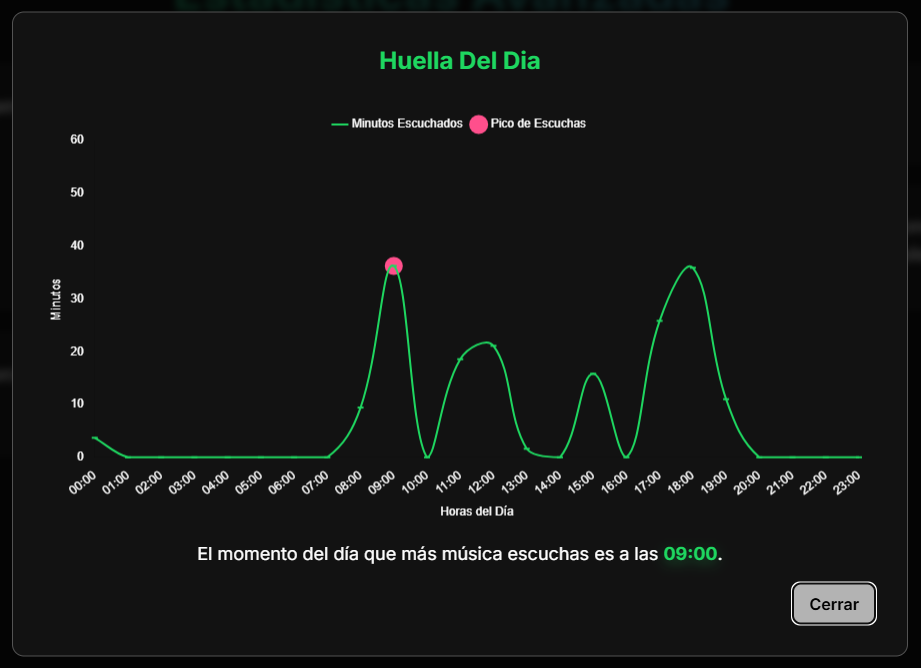
\includegraphics[width=0.55\textwidth]{figures/capturas_ui/huella_del_dia.png}
    \caption{Interfaz de la estadística \textit{Huella Del Día}.}
    \label{fig:huella_del_dia}
\end{figure}

\begin{figure}[H]
    \centering
    \vspace{-10pt}
    \begin{minipage}{0.47\textwidth}
        \centering
        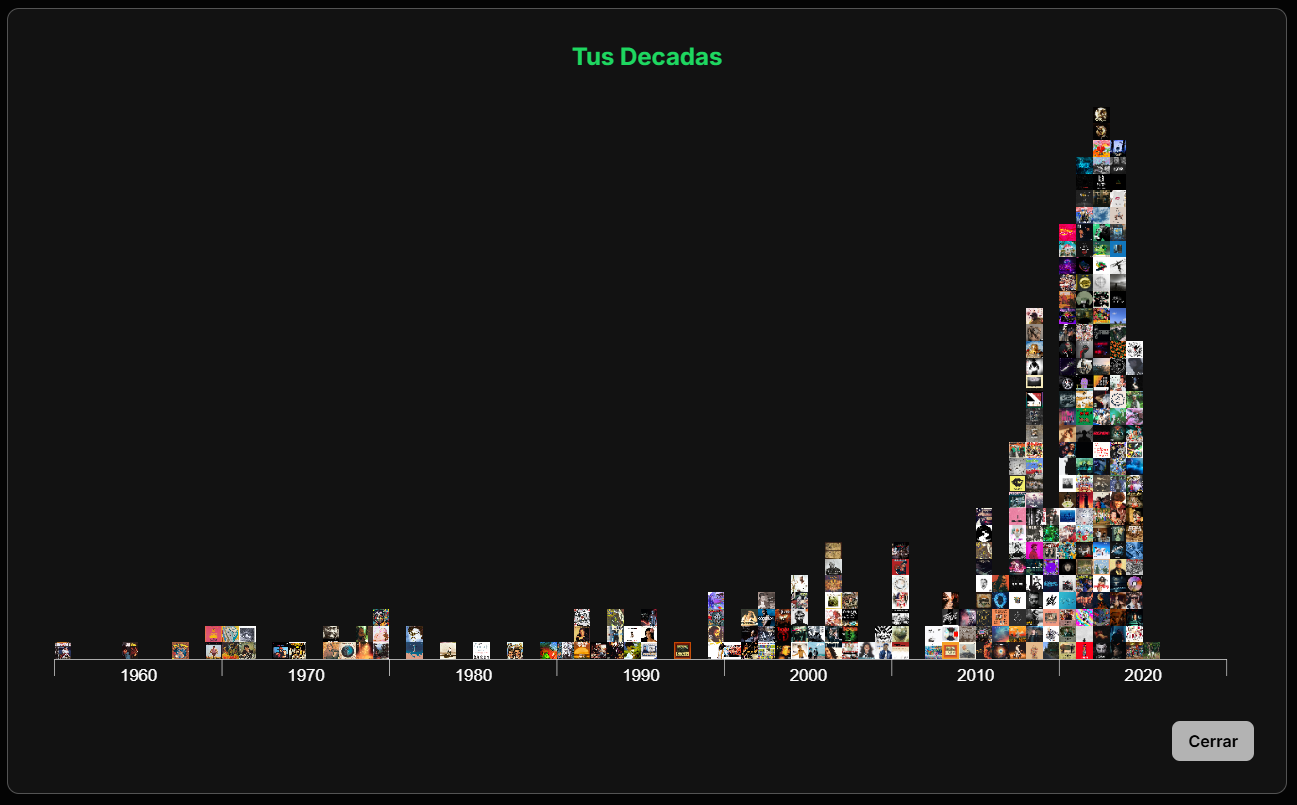
\includegraphics[width=\textwidth]{figures/capturas_ui/tus_decadas_out.png}
        \caption{Interfaz de la estadística \textit{Tus Décadas} (zoom out).}
        \label{fig:tus_decadas_out}
    \end{minipage}
    \begin{minipage}{0.47\textwidth}
        \centering
        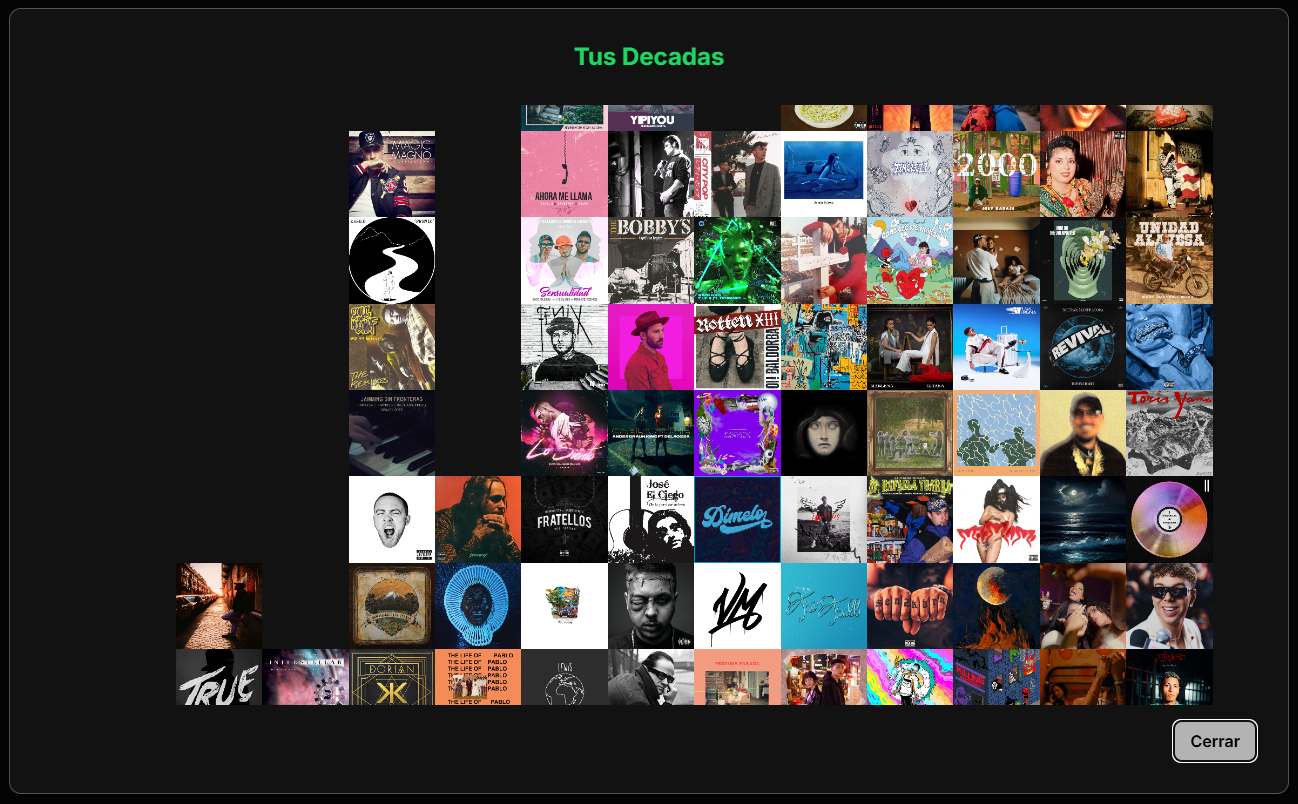
\includegraphics[width=\textwidth]{figures/capturas_ui/tus_decadas_zoom.png}
        \caption{Interfaz de la estadística \textit{Tus Décadas} (zoom in).}
        \label{fig:tus_decadas_zoom}
    \end{minipage}
    \caption{Interfaz de la estadística \textit{Tus Décadas}, en diferentes niveles de zoom.}
    \label{fig:tus_decadas}
\end{figure}

\begin{figure}[H]
    \centering
    \vspace{-10pt}
    \begin{minipage}{0.47\textwidth}
        \centering
        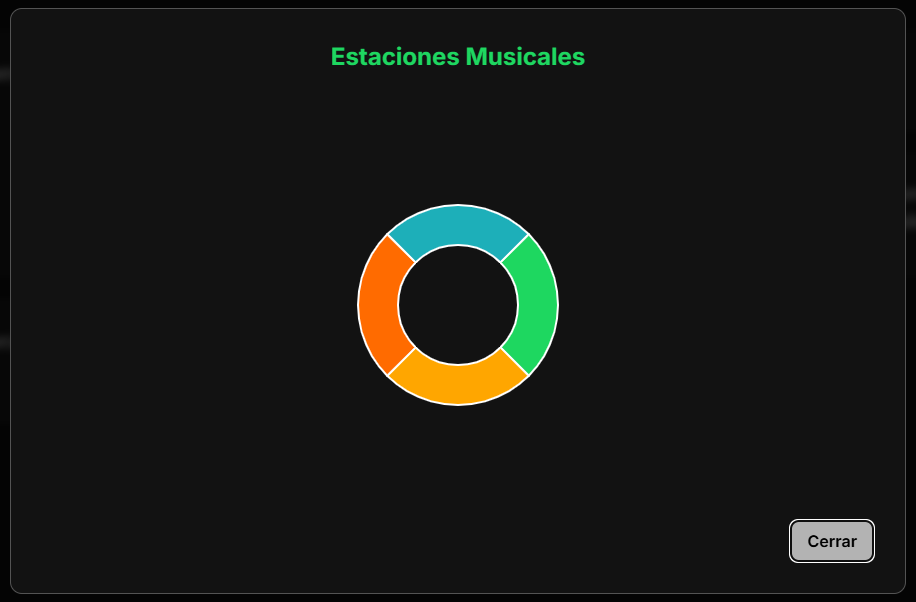
\includegraphics[width=\textwidth]{figures/capturas_ui/estaciones_musicales_cerrado.png}
        \caption{Interfaz de la estadística \textit{Estaciones Musicales} (cerrado).}
        \label{fig:estaciones_musicales_cerrado}
    \end{minipage}
    \begin{minipage}{0.47\textwidth}
        \centering
        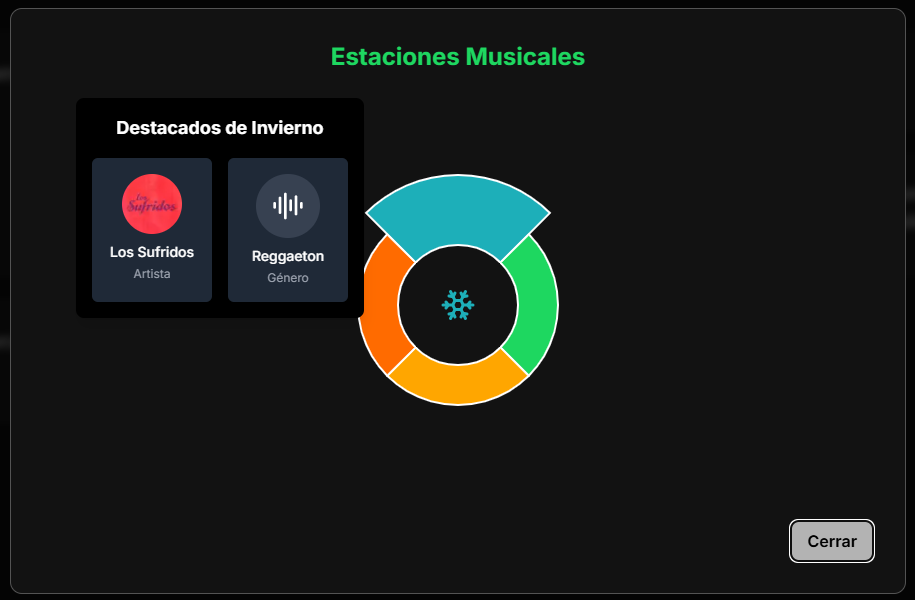
\includegraphics[width=\textwidth]{figures/capturas_ui/estaciones_musicales_abierto.png}
        \caption{Interfaz de la estadística \textit{Estaciones Musicales} (abierto).}
        \label{fig:estaciones_musicales_abierto}
    \end{minipage}
    \caption{Interfaz de la estadística \textit{Estaciones Musicales}, en los estados de cerrado y abierto.}
    \label{fig:estaciones_musicales}
\end{figure}

\begin{figure}[H]
    \centering
    \vspace{-10pt}
    \begin{minipage}{0.47\textwidth}
        \centering
        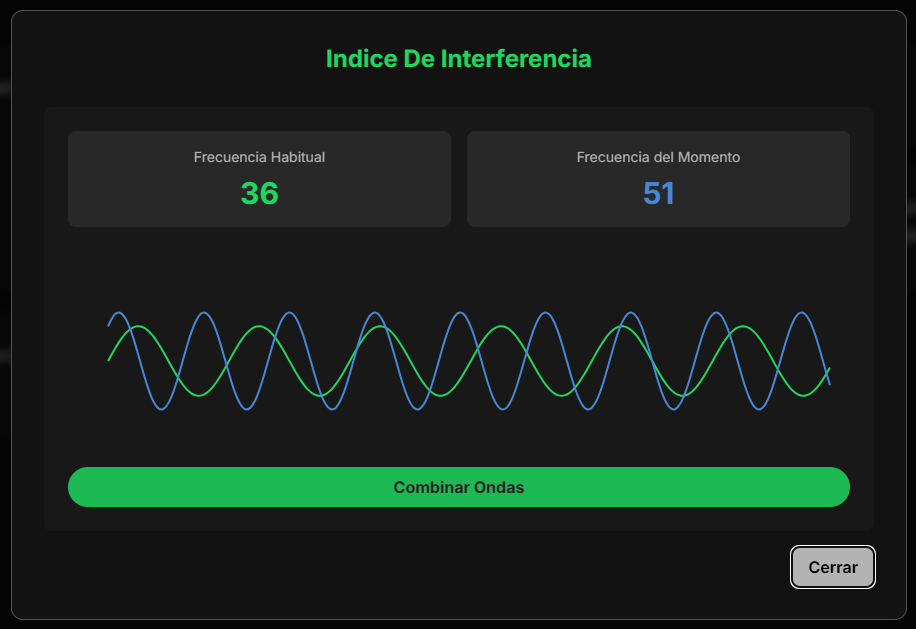
\includegraphics[width=\textwidth]{figures/capturas_ui/indice_de_interferencia_originales.png}
        \caption{Interfaz de la estadística \textit{Índice De Interferencia} (originales).}
        \label{fig:indice_de_interferencia_originales}
    \end{minipage}
    \begin{minipage}{0.47\textwidth}
        \centering
        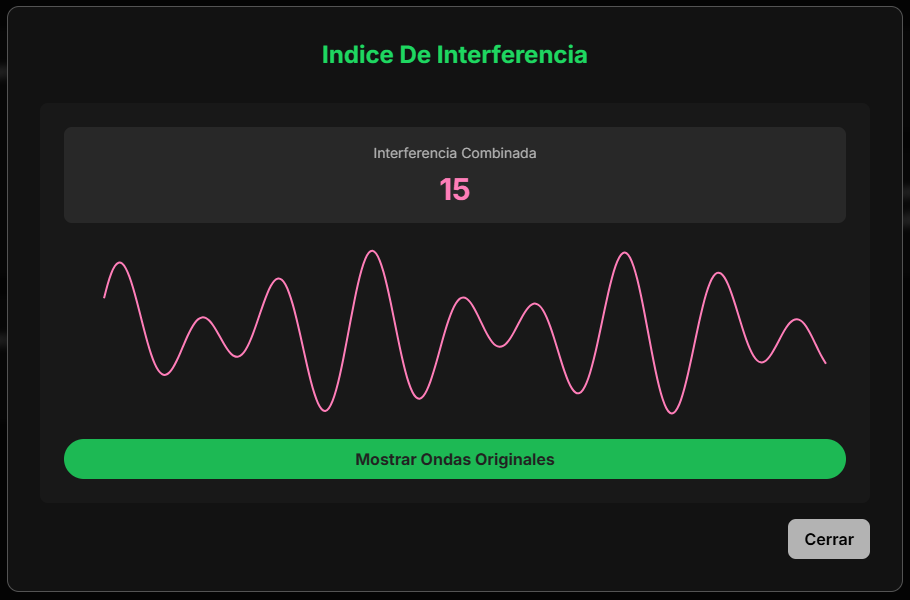
\includegraphics[width=\textwidth]{figures/capturas_ui/indice_de_interferencia_combinado.png}
        \caption{Interfaz de la estadística \textit{Índice De Interferencia} (combinados).}
        \label{fig:indice_de_interferencia_combinado}
    \end{minipage}
    \caption{Interfaz de la estadística \textit{Índice De Interferencia}, con las ondas originales y su forma combinada.}
    \label{fig:indice_de_interferencia}
\end{figure}

\section{Componentes Secundarios, de Carga y de Errores}

Además de los elementos presentados, también se han implementado algunos componentes secundarios para aportar más interactividad a la web y mejorar la experiencia al usuario.

\begin{figure}[H]
    \centering
    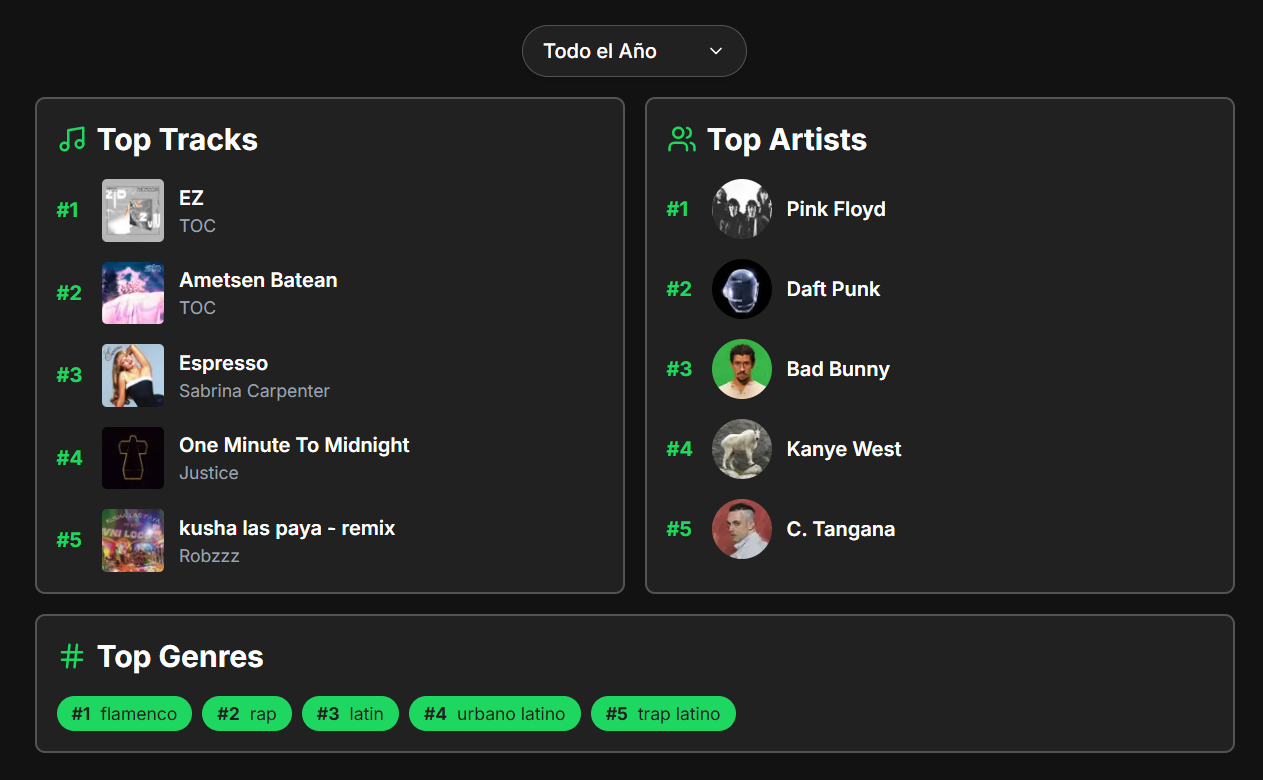
\includegraphics[width=0.75\textwidth]{figures/capturas_ui/tops_detalle.png}
    \caption{Detalle de los tres \textit{tops} junto con el selector de periodo de tiempo.}
    \label{fig:tops_detalle}
\end{figure}

\begin{figure}[H]
    \centering
    \vspace{-10pt}
    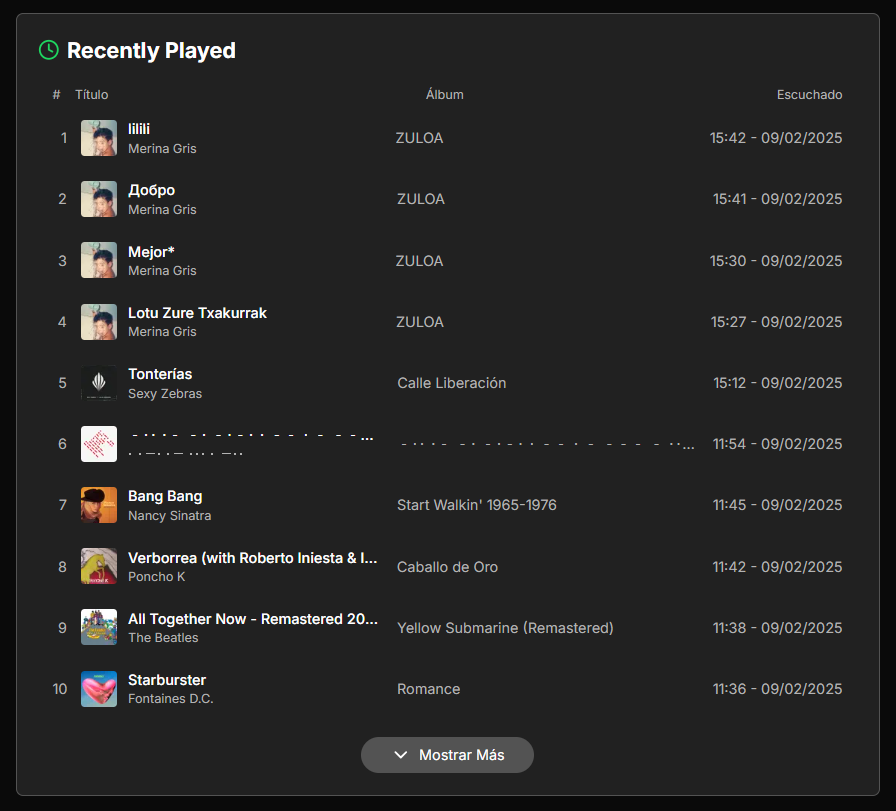
\includegraphics[width=0.75\textwidth]{figures/capturas_ui/recently_played.png}
    \caption{Detalle de \textit{Recently Played} con el botón para ampliar o contraer la lista.}
    \label{fig:recently_played}
\end{figure}

\begin{figure}[H]
    \centering
    \vspace{-10pt}
    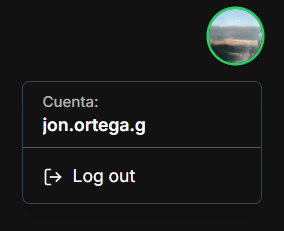
\includegraphics[width=0.4\textwidth]{figures/capturas_ui/user_action_panel.png}
    \caption{Panel del usuario con la opción de \textit{Log Out}.}
    \label{fig:user_action_panel}
\end{figure}

\begin{figure}[H]
    \centering
    \vspace{-10pt}
    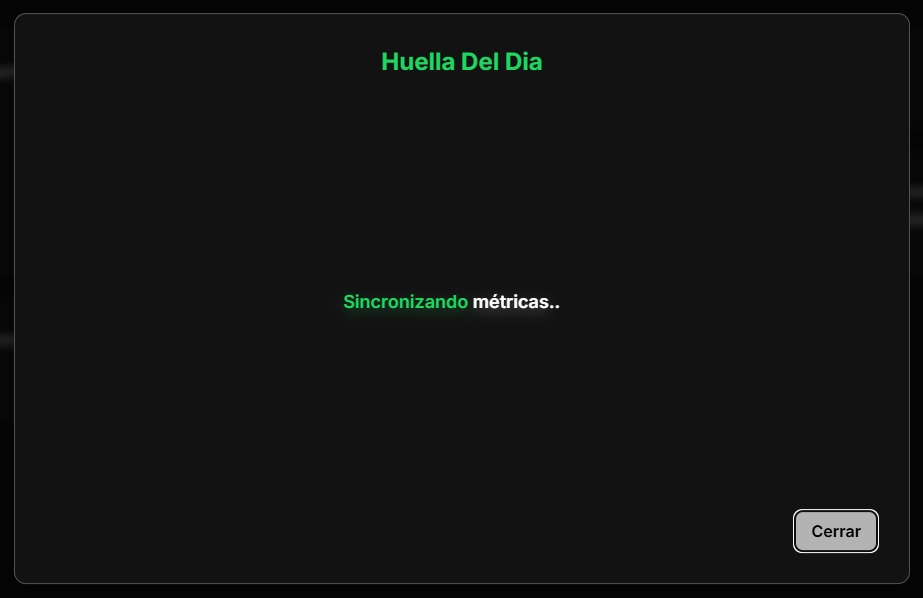
\includegraphics[width=0.75\textwidth]{figures/capturas_ui/pantalla_carga.png}
    \caption{Componente que se muestra mientras se cargan los datos de las estadísticas, con texto dinámico.}
    \label{fig:pantalla_carga}
\end{figure}

\begin{figure}[H]
    \centering
    \vspace{-10pt}
    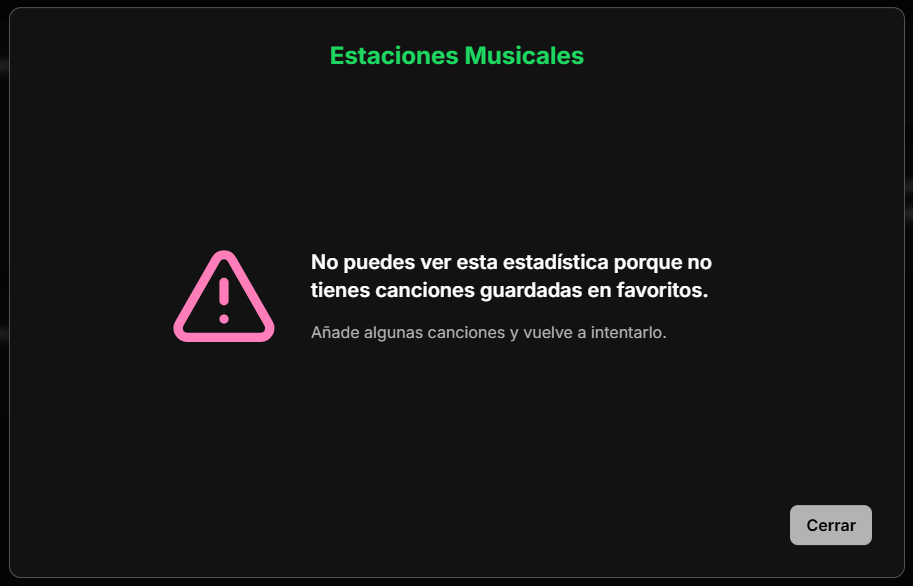
\includegraphics[width=0.75\textwidth]{figures/capturas_ui/error_no_favoritos.png}
    \caption{Componente de error que se muestra cuando el usuario no tiene ninguna canción guardada en su lista de favoritos.}
    \label{fig:error_no_favoritos}
\end{figure}

\begin{figure}[H]
    \centering
    \vspace{-10pt}
    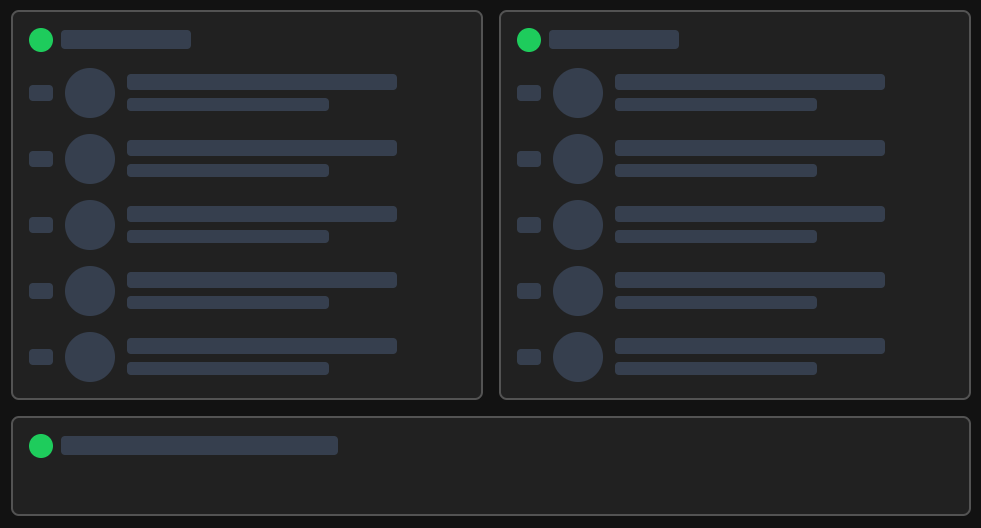
\includegraphics[width=0.8\textwidth]{figures/capturas_ui/skeletons.png}
    \caption{Componentes de \textit{loading} para los tres \textit{tops}.}
    \label{fig:skeletons}
\end{figure}

\chapter{Diagramas de Secuencia Adicionales} \label{ch:anexoB}

\begin{itemize}
    \item \textbf{Cerrar Sesión:} figura \ref{fig:ds_cerrar_sesion}
    \item \textbf{Ver Huella Del Día:} figura \ref{fig:ds_ver_huella_del_dia}
    \item \textbf{Ver Estaciones Musicales:} figura \ref{fig:ds_ver_estaciones_musicales}
    \item \textbf{Ver Tus Décadas:} figura \ref{fig:ds_ver_tus_decadas}
    \item \textbf{Ver Índice de Interferencia:} figura \ref{fig:ds_ver_indice_de_interferencia}
\end{itemize}

\begin{figure}[H]
    \centering
    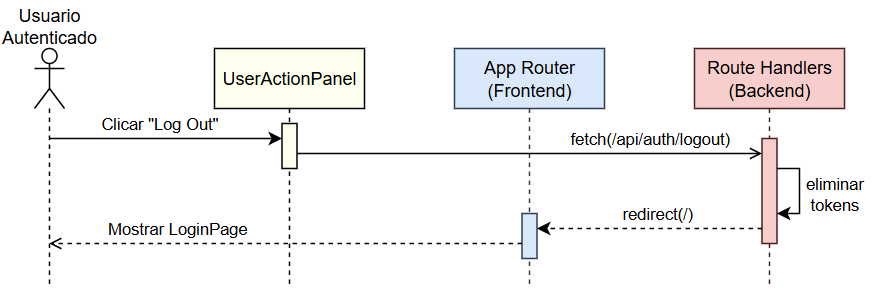
\includegraphics[width=0.85\textwidth]{figures/diagramas_secuencia/ds_cerrar_sesion.png}
    \caption{Diagrama de secuencia: \textbf{Cerrar Sesión}.}
    \label{fig:ds_cerrar_sesion}
\end{figure}

\begin{figure}[H]
    \centering
    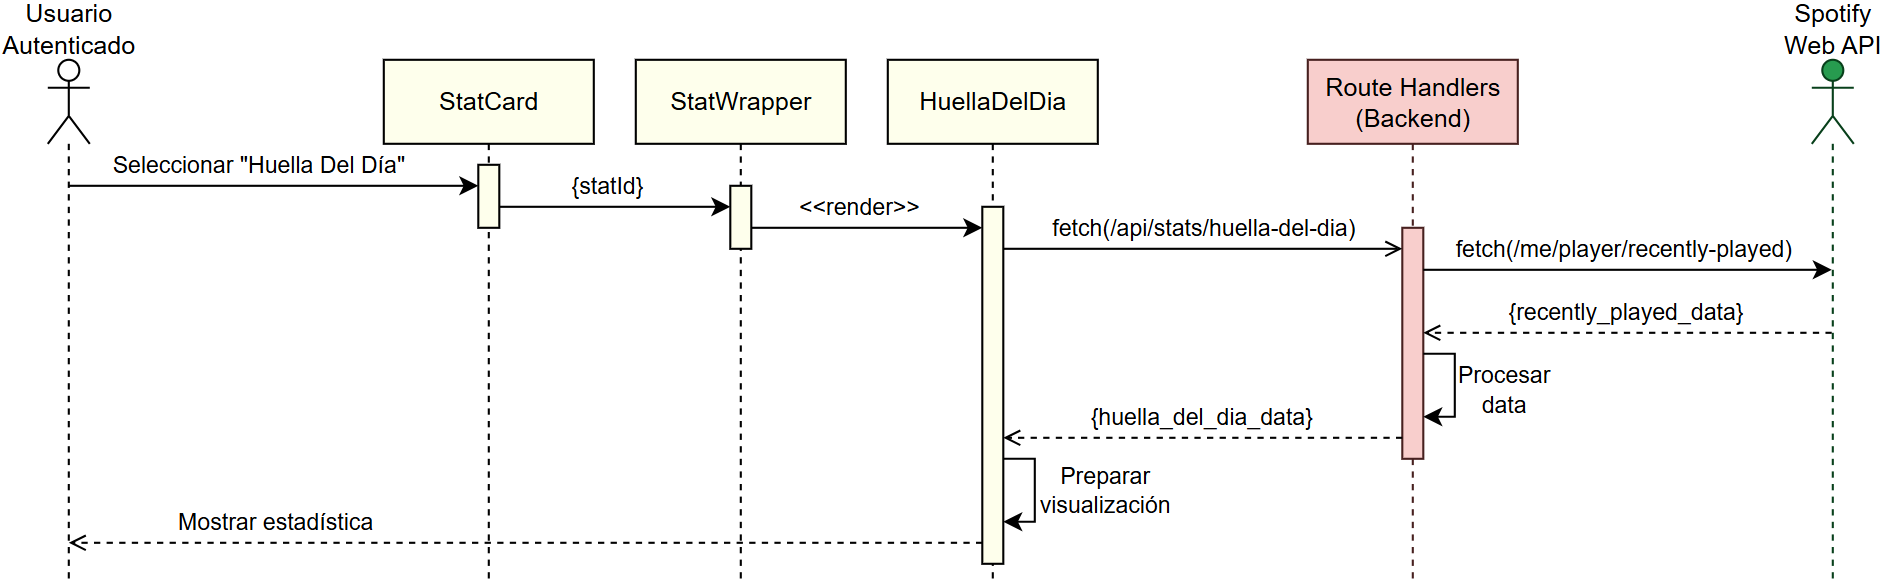
\includegraphics[width=\textwidth]{figures/diagramas_secuencia/ds_ver_huella_del_dia.png}
    \caption{Diagrama de secuencia: \textbf{Ver Huella Del Día}.}
    \label{fig:ds_ver_huella_del_dia}
\end{figure}

\begin{figure}[H]
    \centering
    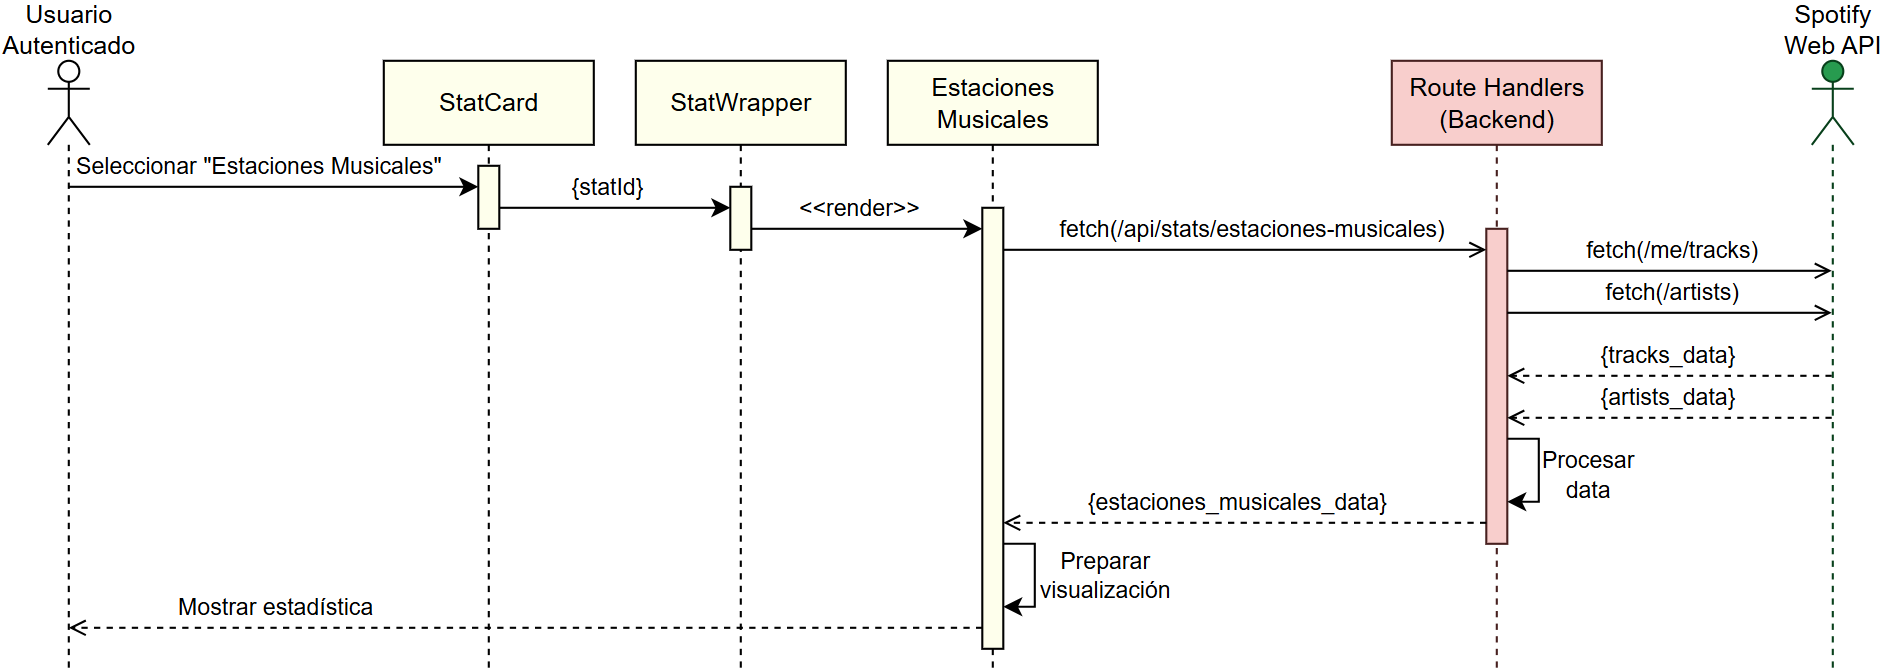
\includegraphics[width=\textwidth]{figures/diagramas_secuencia/ds_ver_estaciones_musicales.png}
    \caption{Diagrama de secuencia: \textbf{Ver Estaciones Musicales}.}
    \label{fig:ds_ver_estaciones_musicales}
\end{figure}

\begin{figure}[H]
    \centering
    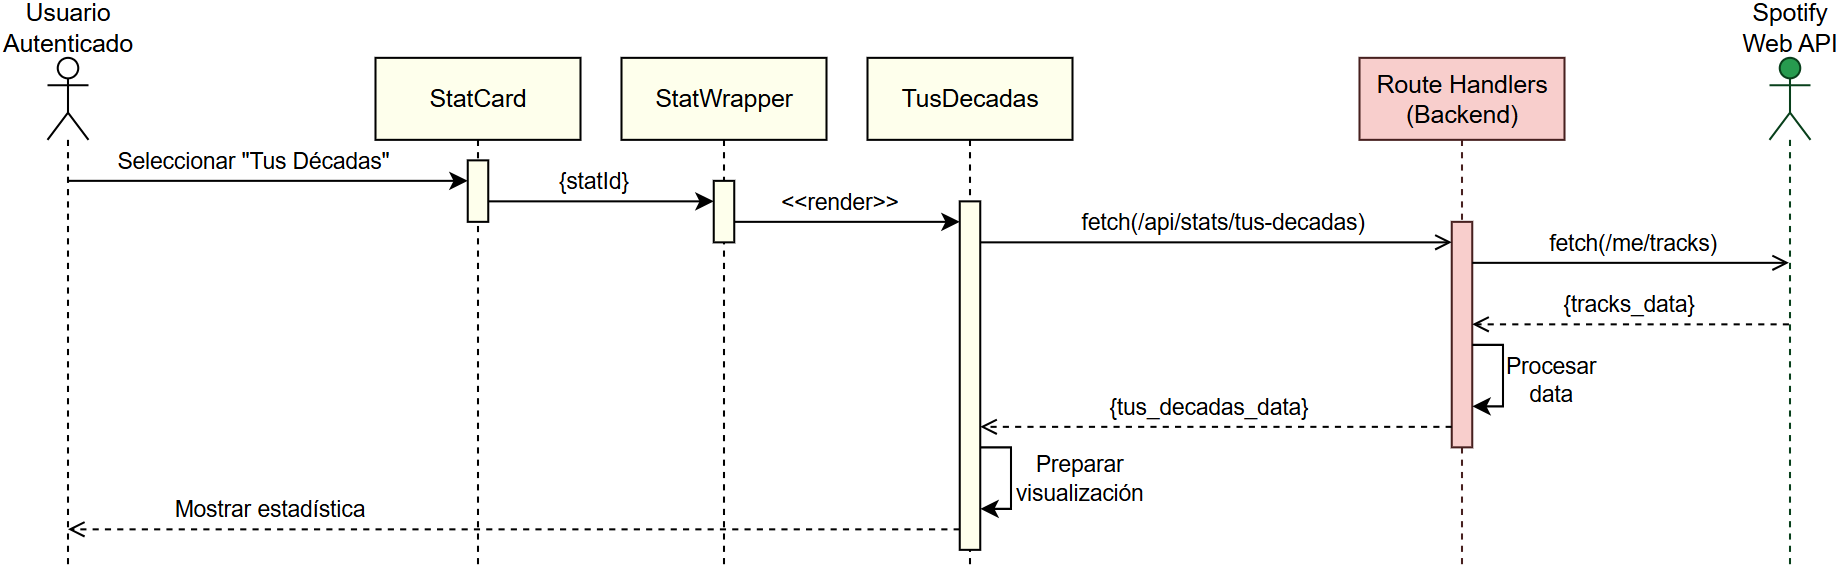
\includegraphics[width=\textwidth]{figures/diagramas_secuencia/ds_ver_tus_decadas.png}
    \caption{Diagrama de secuencia: \textbf{Ver Tus Décadas}.}
    \label{fig:ds_ver_tus_decadas}
\end{figure}

\begin{figure}[H]
    \centering
    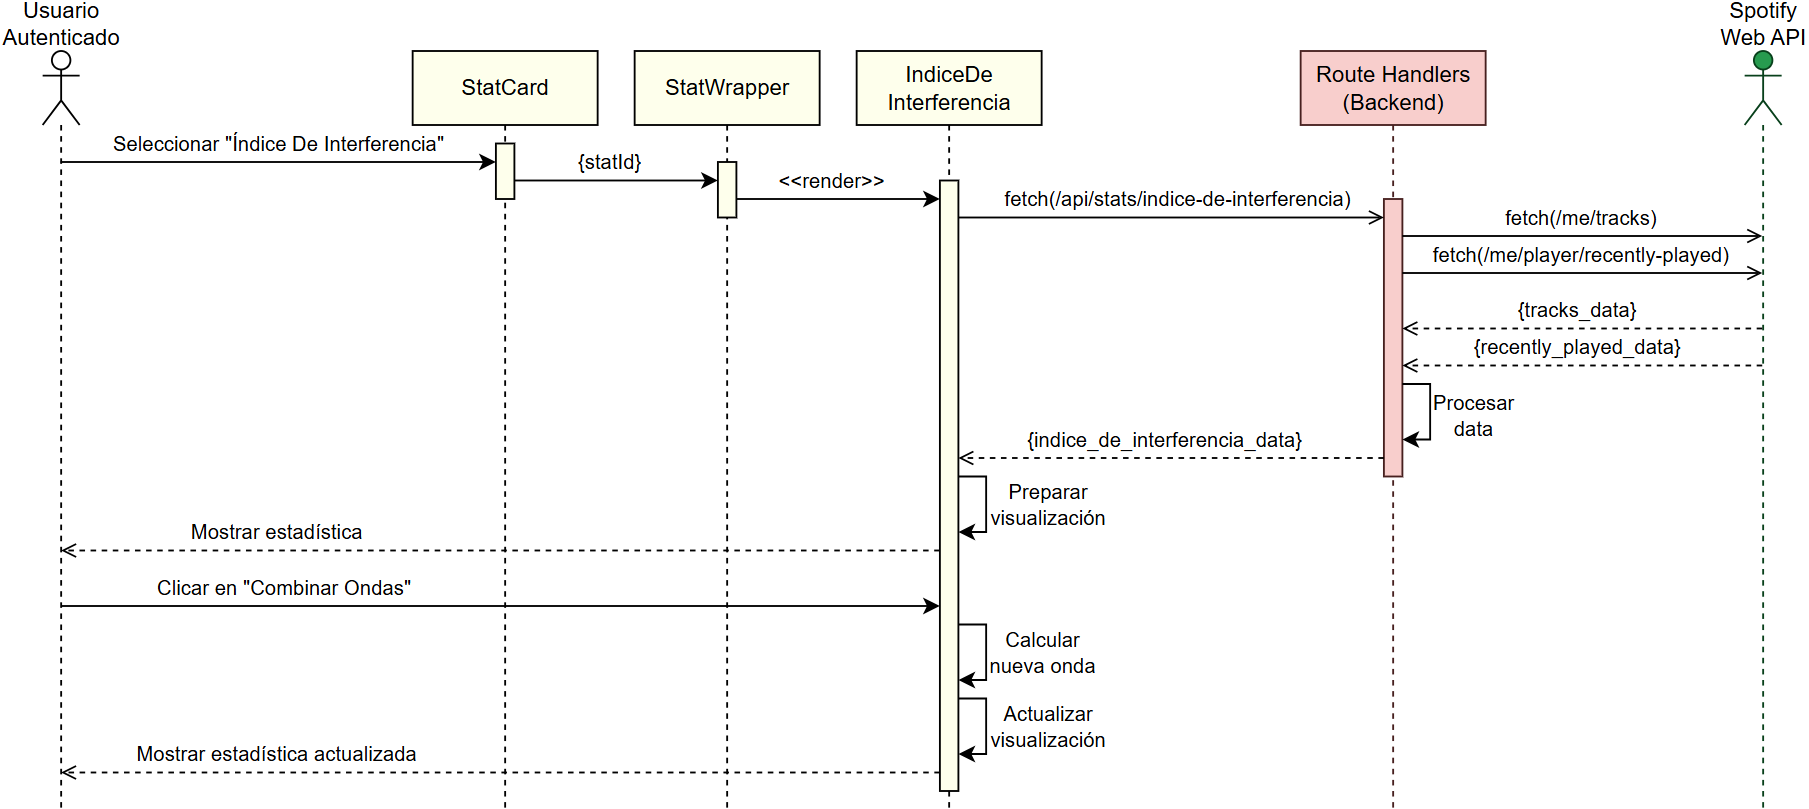
\includegraphics[width=\textwidth]{figures/diagramas_secuencia/ds_ver_indice_de_interferencia.png}
    \caption{Diagrama de secuencia: \textbf{Ver Índice De Interferencia}.}
    \label{fig:ds_ver_indice_de_interferencia}
\end{figure}

\chapter{Ficheros Relacionados con la Implementación} \label{ch:anexoC}

\section{Fichero .env.local}

\begin{ifalgorithm}[H]
    \begin{lstlisting}[language=bash]
    # ID del cliente registrado en la API de Spotify
    SPOTIFY_CLIENT_ID="81af...642b"

    # Secreto del cliente registrado en la API de Spotify no compartir nunca
    SPOTIFY_CLIENT_SECRET="1207...393e"

    # URL del dominio donde se ejecuta la aplicacion en desarrollo, localhost
    DOMAIN_URL="http://localhost:3000"

    # URI de redireccion configurada en Spotify para la autenticacion OAuth
    SPOTIFY_REDIRECT_URI="http://localhost:3000/api/auth/callback"

    # URL utilizada por NextAuth para gestionar la autenticacion en la aplicacion
    NEXTAUTH_URL="http://localhost:3000/api/auth/callback"
    \end{lstlisting}
    \caption{Variables de entrono necesarios en el fichero \texttt{.env.local}.}
    \label{alg:variables_entorno}
\end{ifalgorithm}


